\chapter{Introduction}

Science case

Galaxy Clusters

IMF

DM fraction in comparison with the IMF 

Studying the matter distribution given by strong gravitational lensing can give us informarion about the iMF of the BCGs

Old stuff

mass to light ratio of 4

percentage of dark matter will allow me to define the IMF more precisely. I want to see what fraction of the mass, what fraction of the surface density is stars

make a plot of the mass as a function of the radius of the cluster 

strong lensing at different radii is usefull.

if I got to certeain radius I will have more dark matter, becaue light drops quickly. 

given my scicne case, am I maybe too pesimistic? shjould I look inside the Eeinstin radius? we want to know what radius we should be looking at, for that we can make a plot for a cluster with typical parameters, 

basically find how much dark matter and hoy many stars are there in the profile

first step, find the luminosity of the cluster

let's take the case of ABELL1068, it's magnitude in U is 21.94, in I is 18.46, in g is 20.09, in r is 19.5

the distance to the galaxy is 591.42857 Mpc

but using the aparent magnitude and the distance, we get  L=2.9631e+9

from the NASA webpage: 1.41e+45	

salpeter mass function is $n(M)\propto M^{-2.3}$  

the NFW density profile is 

\begin{equation}
\rho(r)=\frac{\delta_{c}\rho_{c}}{(r/r_{s})(1+r/r_{s})^{2}}
\end{equation}

where the characteristic overdensity is:

\begin{equation}
\delta_{c}=\frac{200}{3}\frac{c^{3}}{\ln{(1+c)}-c/(1+c)}
\end{equation}

from Munoz cuartas et. al. we see that the concentration parameter depends on the mass and the redshift as we see in the following plot:

\begin{figure}[H]
\centering
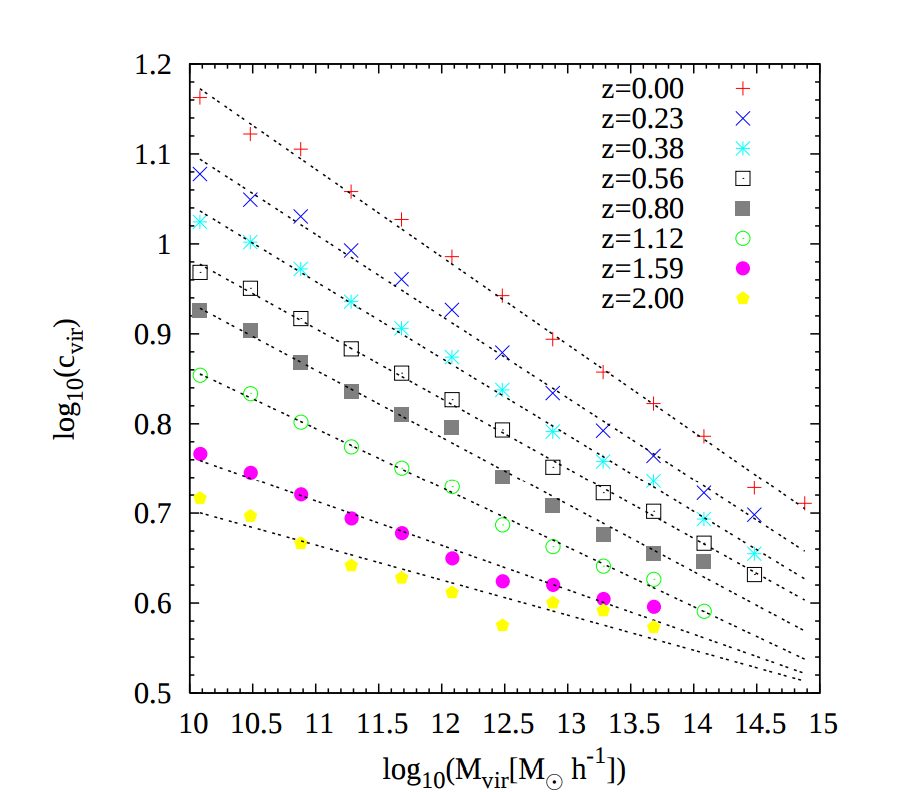
\includegraphics[width=12cm]{images/juank.png}
\caption[M]{G}
\end{figure}
juank.png

(grafica de Juank)

then the concentration parameter for ABELL1068 is about 4.46 

so from the critical density:

\begin{equation}
\rho_{c}=\frac{3H^2(z)}{8\pi G}
\end{equation}

the critical desntiy would be: 2e-26 in SI units so in Msol/pc3 it is $2.9\times 10^{-7}$

$H(z)=H_{0}(1+\Omega z)^{3/2}$

the hubble parameter at z=0.138 is H(z)=85.6

let's take a value of 40 kpc for the concentration parameter given by $r_{s}=r_{200}/c$

delta c is 6716.38



\newpage
